%! Author = Filippo Vissani
%! Date = 08/02/24
% !TeX root = ../thesis-main.tex

%----------------------------------------------------------------------------------------
\chapter{Design}
\label{chap:design}
%----------------------------------------------------------------------------------------

\section{Architecture}

\subsection{Purely Reactive Model}

\begin{figure}
    \centering
    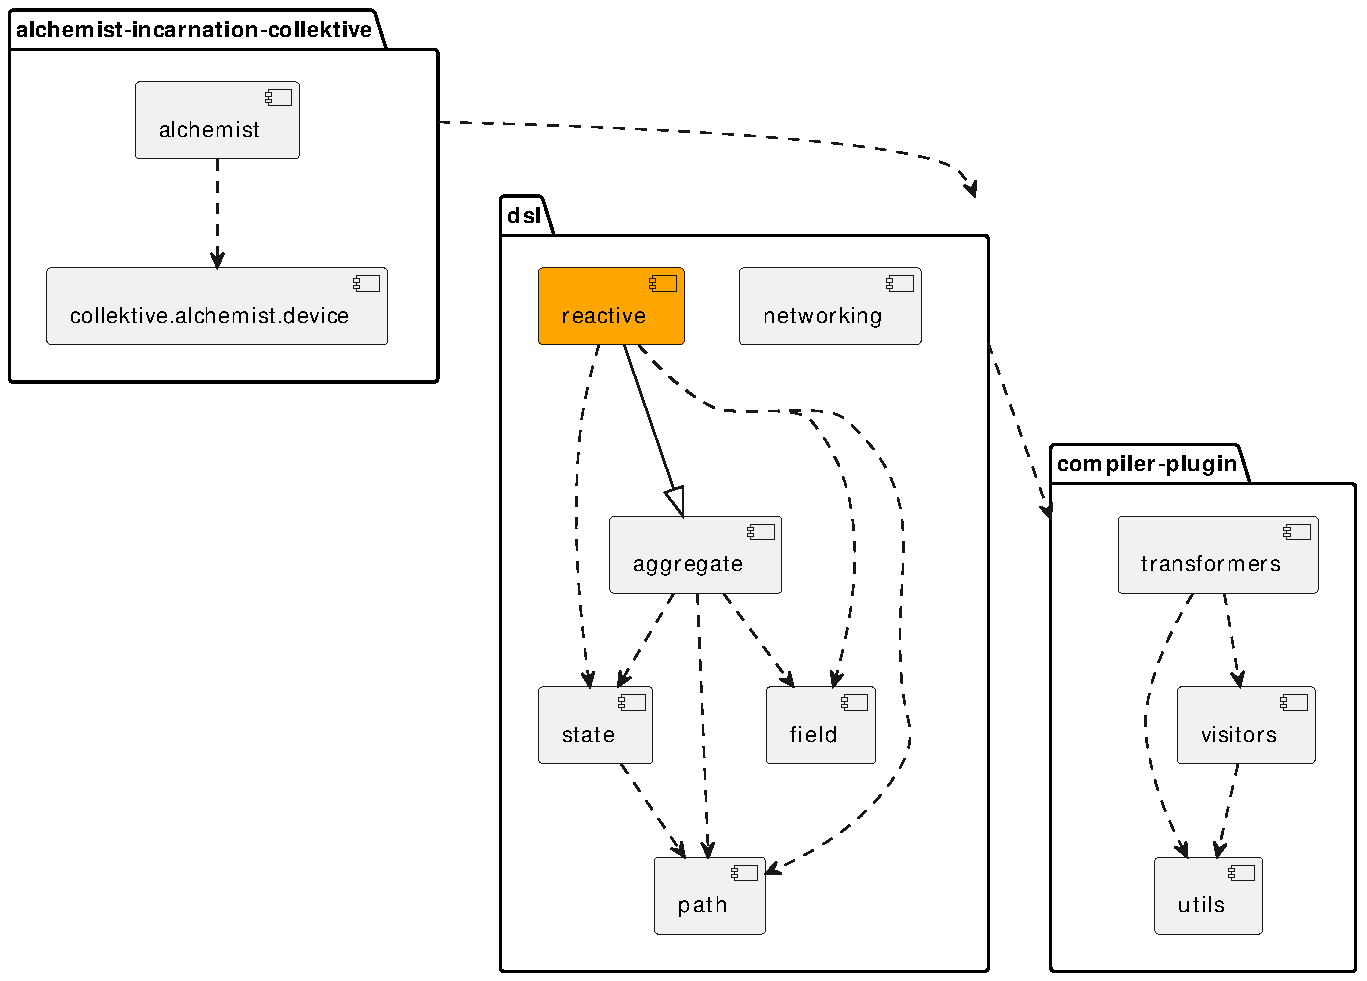
\includegraphics[width=\linewidth]{figures/collektive-prm-architecture.pdf}
    \caption{Architecture of the purely reactive model proposed.}
    \label{fig:collektive-prm-architecture}
\end{figure}

\subsection{Model with Reactive Messages and Sensors}

\section{Detailed Design}

\subsection{Purely Reactive Model}

\begin{figure}
    \centering
    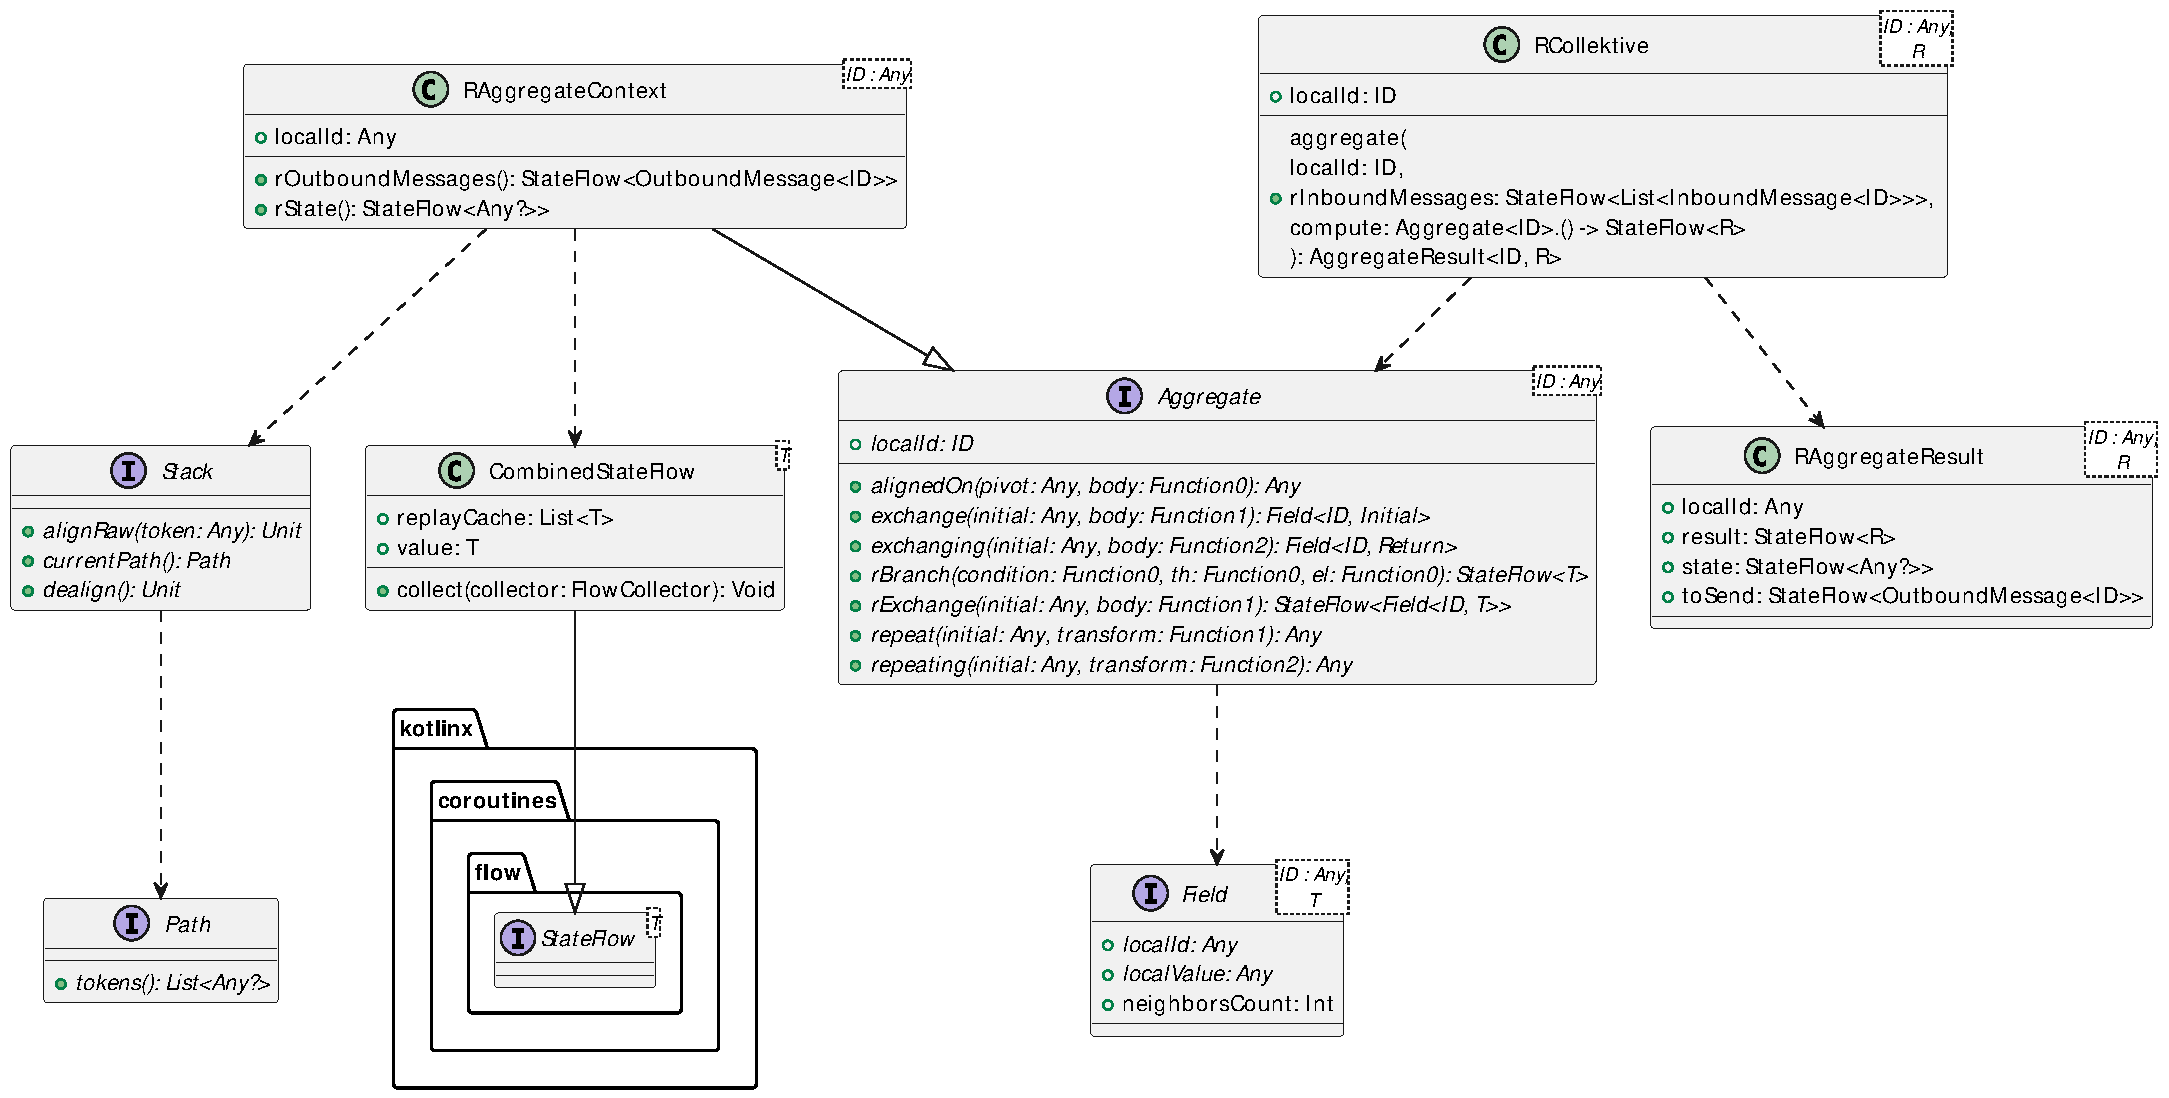
\includegraphics[width=\linewidth]{figures/collektive-prm-design.pdf}
    \caption{Detailed design of the purely reactive model proposed.}
    \label{fig:collektive-prm-design}
\end{figure}

\subsection{Model with Reactive Messages and Sensors}

\begin{figure}
    \centering
    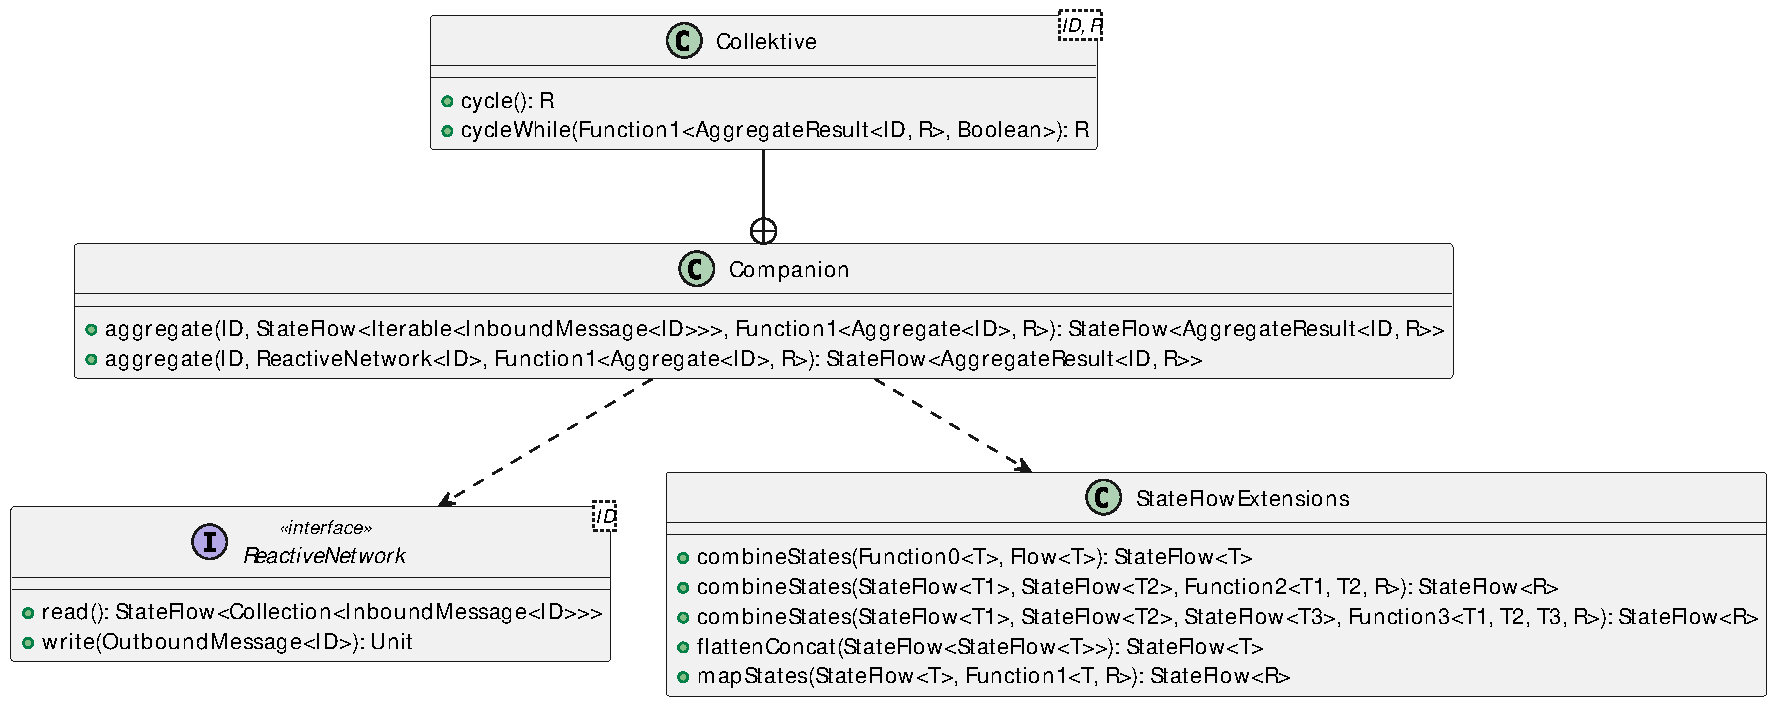
\includegraphics[width=\linewidth]{figures/collektive-rmsm-design.pdf}
    \caption{Detailed design of the model with reactive messages and sensors.}
    \label{fig:collektive-rmsm-design}
\end{figure}
